\chapter{Evaluation}\label{chap:6}


\section{Accuracy evaluation}
In 935 malware PE files obtained, 635 of them are to make eight decision trees. 200 malware meta-data in training data is applied to, in order to sort $8$ decision tree, and to make the best order of decision tree as shown in Figure \ref{fig:ordertree}, this order has the best experimental result with ? malware training data. 
Finally, Lasrly, 100 remaining malware meta-data are kept to test experimental result the system.
Experiment results in the order of decision tree given	 in Figure \ref{fig:ordertree}.
\begin{figure}[httb]
  \centering
    
\includegraphics[width=1\textwidth]{graph/ordertree.jpg}
     \caption{The best decision tree order.}
     \label{fig:ordertree}
\end{figure}

In the decision tree order, 100 malware are taken to check the experimental result of system, and Table \ref{fig:experimentalresult} reveals that result. Some of data in axis show these total number of malware in that family, and that number is separated into groups that these malware has been classified by the system. For example, there are four malwares in Win32/Virut family, and three of them are successfully sorted into Win32/Virut family and, while one malware is in other family. Therefore, the system recognizes the trojan agent family with 75 \% of accuracy.\\
\\

\begin{figure}[h!]
  \begin{center}
    \begin{tabular}{ | l | l | l | l | l | l | l | l | l | l |}
     \hline
    Malware & Virut & Autorun & IRCbot & Gaobot & Waledac & Downadup & Sality & Mota & Accuracy\\ \hline
    Virut & ? & ? & ? & ? & ? & ? & ? & 75\% \\ \hline
	Autorun & 0 & 0 & 0 & ? & ? & ? & ? & 50\% \\ \hline
	IRCbot & 0 & 0 & 2 & 0 & 1 & 0 & 0 & 66\% \\ \hline
	Gaobot & 1 & 0 & 0 & 2 & 8 & 0 & 3 & 53\% \\ \hline
	Waledac & 0 & 0 & 0 & 0 & 0 & 0 & 0 & 0\% \\ \hline
	Downadup & 0 & 0 & 0 & 0 & 0 & 1 & 1 & 50\% \\ \hline
	Sality & 0 & 0 & 0 & 0 & 0 & 1 & 1 & 50\% \\ \hline
	Mota & 4 & 4 & 2 & 3 & 15 & 2 & 41 & 57\% \\ \hline

    \end{tabular}
	\end{center}
     \caption{Experimental result}
    \label{fig:experimentalresult}
\end{figure} 

The system is useful to help virus researcher determine the malware family that unknown malware belongs to. The malware family contains Win32/Virut, Win32/Autorun, Win32/IRCbot, Win32/Gaobot, Win32/Waledac, Win32/Downadup, Win32/Sality, W32.Mota, known as famous malware family. Virus researchers who know the family of malware can easily find out some semantic similarities between malwares and shows their inner similarity in behavior and static malware characteristics.

\section{Efficiency of classifying}
Figure show comparing the step to detect semantic malware characterization using Virus total with our approach.
 \begin{figure}[httb]
  \centering
    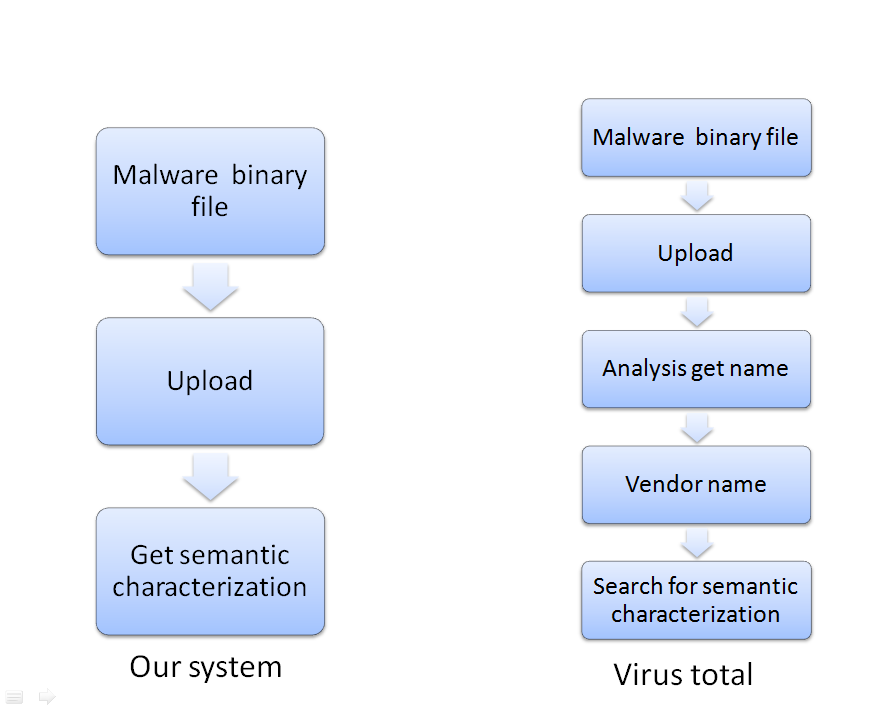
\includegraphics[width=1\textwidth]{graph/evaluation3.png}
     \caption{The best decision tree order.}
     \label{fig:evaluation3}
\end{figure}

The figure 1 show classifying time in our system. The evaluation was performed on a 2.4 HZ core i3 laptop with 4G memory, running in ubuntu 11.4. 	

\begin{figure}[httb]
  \centering
    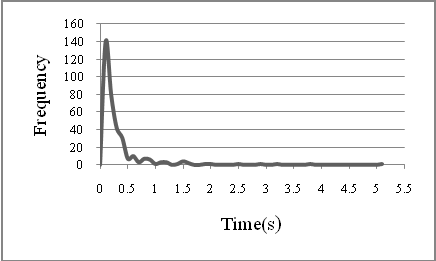
\includegraphics[width=1\textwidth]{graph/evaluation2.png}
     \caption{The best decision tree order.}
     \label{fig:evaluation2}
\end{figure}
The result was shown in figure \ref{fig:evaluation1}. The median time to perform classification was 0.25 seconds. The slowest sample classified required 5.12 seconds. Only 6 samples required more than 2 seconds. Processing time of followgraph approach was shown in figure \ref{fig:evaluation2}.

